La méthode de partage de poids dite « douce », quant à elle, ne modifie pas la structure-même du réseau.
Elle se base sur l'expression d'une métrique de contrainte entre les poids des noyaux des deux couches morphologiques du réseau, qui est alors ajoutée dans la fonction de perte globale \textit{loss}, et qui va ainsi faire tendre ces deux noyaux symétriquement vers la même forme durant l'entraînement du réseau, sans donc passer par un transfert direct dur des poids d'une couche à l'autre. 
La contrainte fait ainsi prendre la même forme aux deux noyaux, mais de manière plus douce. \\
%La << puissance >> de cette contrainte par rapport aux autres métriques dans la \textit{loss} est modulée par un hyperparamètre noté $\lambda$. \\

\vspace{-2.0mm}
Rappelons d'abord la formule de l'erreur quadratique moyenne (MSE) entre deux fonctions $f_1$ et $f_2$ définies sur le même ensemble dénombrable $I$ à valeurs dans $\mathbb{R}$, qui est utilisée dans notre cas pour calculer l'éloignement entre deux images : \\

\vspace{-4.4mm}
\begin{equation}
    \text{MSE} (f_1,f_2) = \mathbb{E} \left ( (f_2-f_1)^2 \right ) = \frac{1}{|I|} \sum_{x \in I} \left ( f_2(x) - f_1(x) \right ) ^2
    \label{MSE}
\end{equation}

\vspace{2.5mm}
La fonction de perte \textit{loss} du réseau, qui permet d'entraîner et d'évaluer les performances de prédiction de ce dernier, se formule classiquement comme la MSE entre les images cibles $F_\text{cible}$ et les images prédites par le réseau $F_\text{pred}$ : $\textit{loss} = \text{MSE}(F_\text{cible},F_\text{pred})$. 
Dans la \textit{loss}, est alors ici ajoutée à $\text{MSE}(F_\text{cible},F_\text{pred})$ une contrainte de similarité $C_\text{sim}$ entre le noyau de la première couche, $w_1$, et celui de la seconde, $w_2$. 
Cette contrainte est pondérée par l'hyperparamètre $\lambda$ qui permet de moduler son influence dans la convergence du réseau lors de l'entraînement, par rapport à celle de $\text{MSE}(F_\text{cible},F_\text{pred})$. \\

\vspace{-2.0mm}
\noindent On étudie trois formulations de cette métrique de contrainte entre $w_1$ et $w_2$. Elles sont explicitées à la page suivante. Pour mieux les comprendre, définissons d'abord deux fonctions de rééchelonnage linéaire primaires, la normalisation et la standardisation. \\

\vspace{0.0mm}
On définit la << normalisation >> comme la fonction $\mathfrak{N}_{(a,b)}$ qui à une image $f: I \rightarrow \mathbb{R}$ associe son rééchelonnage linéaire (rescale) dans un intervalle $[a,b] \subset \mathbb{R}$ : \\

\vspace{-3.5mm}
\begin{equation}
    \mathfrak{N}_{(a,b)} (f) = \frac{f-\inf_{x \in I}\{f(x)\}}{\sup_{x \in I}\{f(x)\}-\inf_{x \in I}\{f(x)\}} \left ( b-a \right ) + a
    \label{normalized}
\end{equation}

\vspace{4.5mm}
On définit la << standardisation >> comme la fonction $\mathfrak{S}$ qui à une image $f: I \rightarrow \mathbb{R}$ associe son rééchelonnage linéaire de moyenne $\mathbb{E}(\mathfrak{S}(f)) = 0$ et d'écart-type $\sigma(\mathfrak{S}(f)) = 1$ sur l'ensemble de ses valeurs d'arrivée $f(I)$ : \\

\vspace{-4.0mm}
\begin{equation}
    \mathfrak{S} (f) = \frac{f-\mathbb{E}(f)}{\sigma(f)} = \frac{ f - \frac{1}{|I|} \sum_{x \in I} f(x) }{ \sqrt{ \frac{1}{|I|} \sum_{x \in I} \left ( f(x) - \frac{1}{|I|} \sum_{x \in I} f(x) \right ) ^2 } }
    \label{standardized}
\end{equation}


\newpage

\noindent \textbf{a. Première formulation} \\

\vspace{-1.5mm}
%, avec les poids du noyau $w_1$ de la première couche du réseau et ceux du noyau $w_2$ de la seconde couche,
La première formulation de la métrique de contrainte $C_\text{sim}$ est définie à partir de la MSE entre les deux noyaux $w_1$ et $w_2$, symétrisés l'un par rapport à l'autre et normalisés (\ref{normalized}) entre 0 et 1. Ainsi, $C_\text{sim}$ est définie pour tous noyaux $w_1$ et $w_2$ par : \\

\vspace{-4.7mm}
\begin{equation}
    C_\text{sim}(w_1,w_2) = \text{MSE} \left ( \mathfrak{N}_{(0,1)}(w_1) , \mathfrak{N}_{(0,1)}(\breve{w_2}) \right )
    \label{Csim1}
\end{equation}

\vspace{3.5mm}
\noindent \textbf{b. Deuxième formulation} \\

\vspace{-1.5mm}
%, avec les poids du noyau $w_1$ de la première couche du réseau et ceux du noyau $w_2$ de la seconde couche,
La deuxième formulation de la métrique de contrainte $C_\text{sim}$ est définie à partir de la MSE entre les deux noyaux $w_1$ et $w_2$, symétrisés l'un par rapport à l'autre et cette fois standardisés (\ref{standardized}). Ainsi, $C_\text{sim}$ est définie pour tous noyaux $w_1$ et $w_2$ par : \\

\vspace{-4.7mm}
\begin{equation}
    C_\text{sim}(w_1,w_2) = \text{MSE} \left ( \mathfrak{S}(w_1) , \mathfrak{S}(\breve{w_2}) \right )
    \label{Csim2}
\end{equation}

\vspace{3.5mm}
\noindent \textbf{c. Troisième formulation} \\

\vspace{-1.5mm}
%, entre les poids du noyau $w_1$ de la première couche du réseau et ceux du noyau $w_2$ de la seconde couche,
La troisième formulation de la métrique de contrainte $C_\text{sim}$ est définie à partir de la MSE entre les deux noyaux $w_1$ et $w_2$, symétrisés l'un par rapport à l'autre et standardisés, mais multipliés par l'écart-type des poids d'un des deux noyaux, afin d'éviter de changer et d'influencer, avec un écart relatif, la taille de la gamme des poids des noyaux. $C_\text{sim}$ est alors définie pour tous noyaux $w_1$ et $w_2$ par : \\

\vspace{-4.7mm}
\begin{equation}
    C_\text{sim}(w_1,w_2) = \text{MSE} \left ( \hspace{1mm}  w_1 - \mathbb{E}(w_1) \hspace{1.5mm},\hspace{1.5mm} ( \breve{w_2} - \mathbb{E}(\breve{w_2}) ) \frac{\sigma(w_1)}{\sigma(\breve{w_2})}  \hspace{1mm} \right )
    \label{Csim3}
\end{equation}

\vspace{3.6mm}
\noindent \textbf{Remarque :} \\

\vspace{-1.5mm}
\noindent Si on prend ici la symétrique de $\breve{w_2}$ de $w_2$, c'est parce que, comme précédemment, le problème de symétrie dans l'expression asymptotique de la formule de $\mathcal{S}$MorphTanh (p. 22) nécessite de prendre la symétrie d'un des deux noyaux $w$. 
De plus, si les trois formulations se basent sur un rééchelonnage des noyaux, c'est parce qu'ils peuvent tous deux s'exprimer dans deux intervalles de $\mathbb{R}$ très différents liés à la standardisation en entrée du réseau et au filtre de convolution de taille 1 en sortie. On imagine alors qu'il doit exister une relation linéaire entre la disposition dans $\mathbb{R}$ des poids du premier noyau $w_1$ et la disposition dans $\mathbb{R}$ de ceux du second noyau $w_2$. \\

\vspace{-0.1mm}
\noindent Avec $C_\text{sim}$ définie par l'une des trois formulations présentées (\ref{Csim1}, \ref{Csim2}, \ref{Csim3}), la nouvelle formule de la \textit{loss} dans le cadre de ce partage de poids doux s'écrit ainsi : \\

\vspace{-4.0mm}
\begin{equation}
    \textit{loss} = \text{MSE} \left ( F_\text{cible},F_\text{pred} \right ) + \lambda \times C_\text{sim}(w_1,w_2)
    \label{MSEpConstraintFilters}
\end{equation}


\newpage

\noindent \textbf{Comparaison rapide de résultats de convergence entre ces trois formulations} \\

Pour savoir quelle formulation de la contrainte de similarité $C_\text{sim}$ entre $w_1$ et $w_2$ est la plus adaptée à nos besoins, on exécute plusieurs expériences d'entraînement de réseau $\mathcal{S}$MorphNetTanh à deux couches, avec séparément les trois différentes formulations de $C_\text{sim}$ telles que décrites précédemment, ajoutées dans la \textit{loss}. On observe alors rapidement la forme des deux noyaux $w_1$ et $w_2$ après convergence du réseau. La figure suivante présente les résultats, associés par paires (la première image pour $w_1$, la seconde qui suit pour $w_2$), sur l'ensemble des expériences avec les huit structures cibles, et deux banques d'images (MNIST et FashionMNIST). \\

%figure
\vspace{-0.5mm}
\begin{figure}[ht]
  \begin{center}
      \subfigure[Avec la 1ère formulation]{
          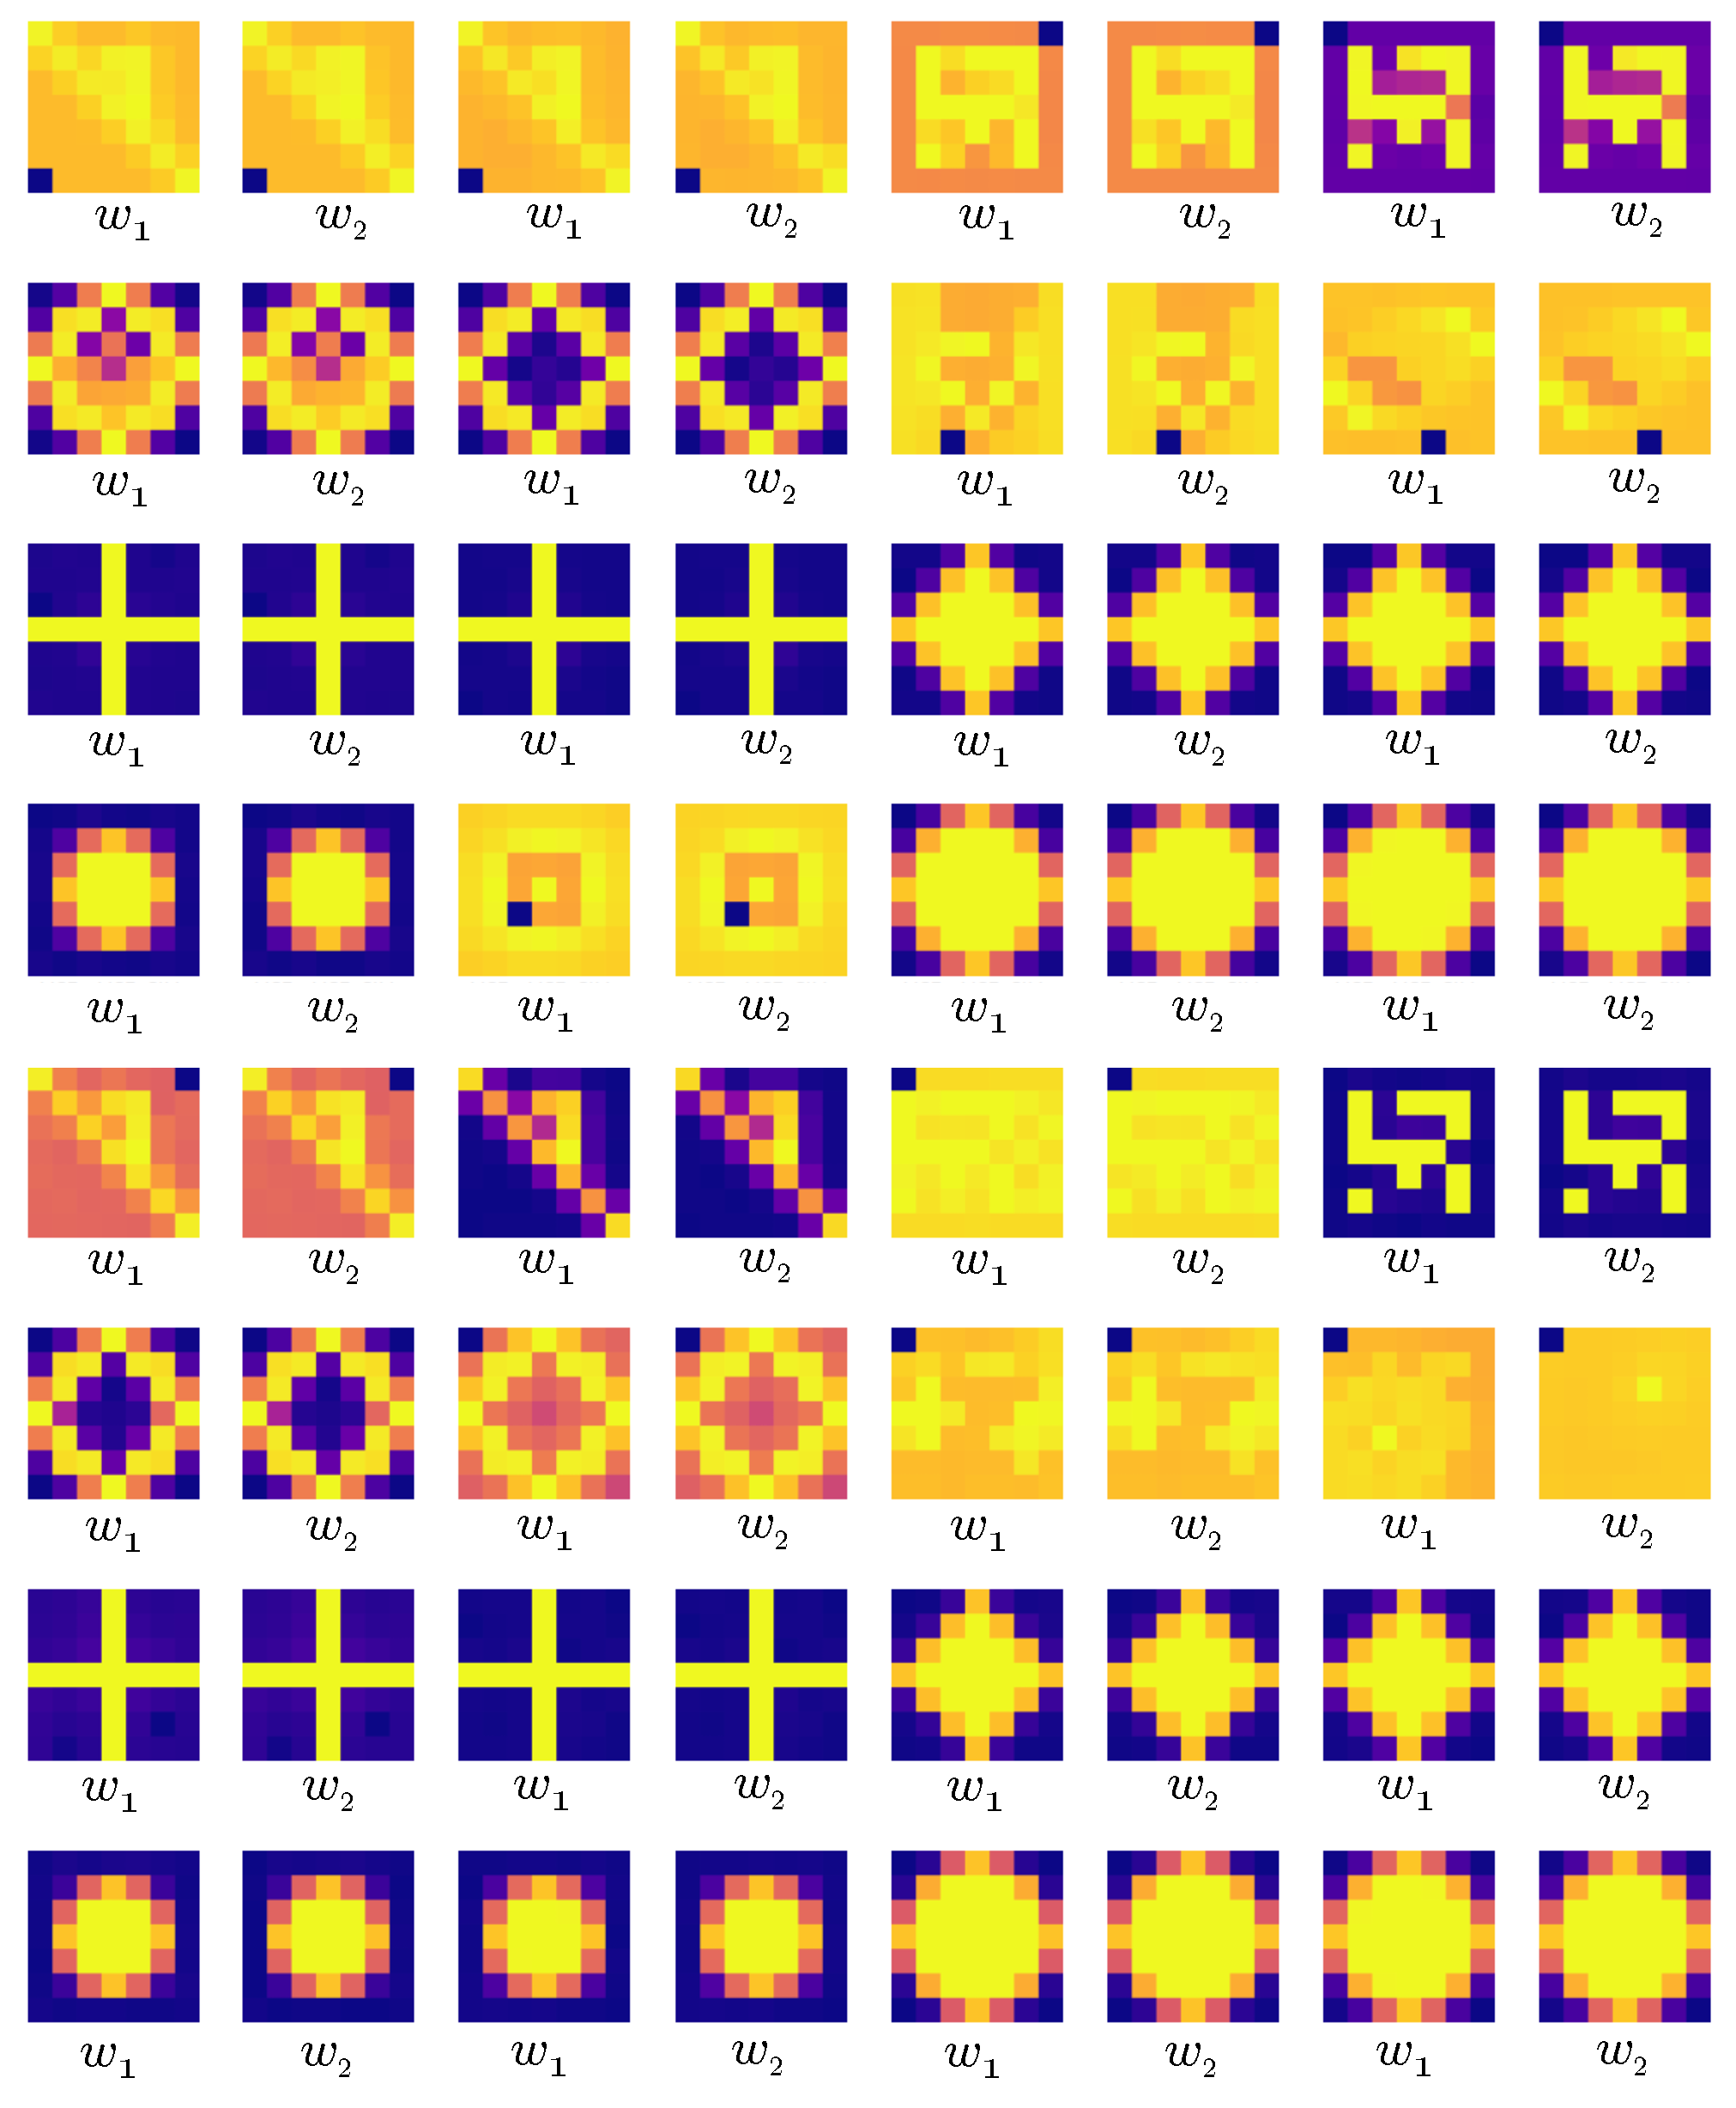
\includegraphics[width=0.31\textwidth]{parts/3-contributions/B-partage_de_poids/figures/quick_visu_NORM.pdf}
          \label{fig:nor1}}\hfill
      \subfigure[Avec la 2ème formulation]{
          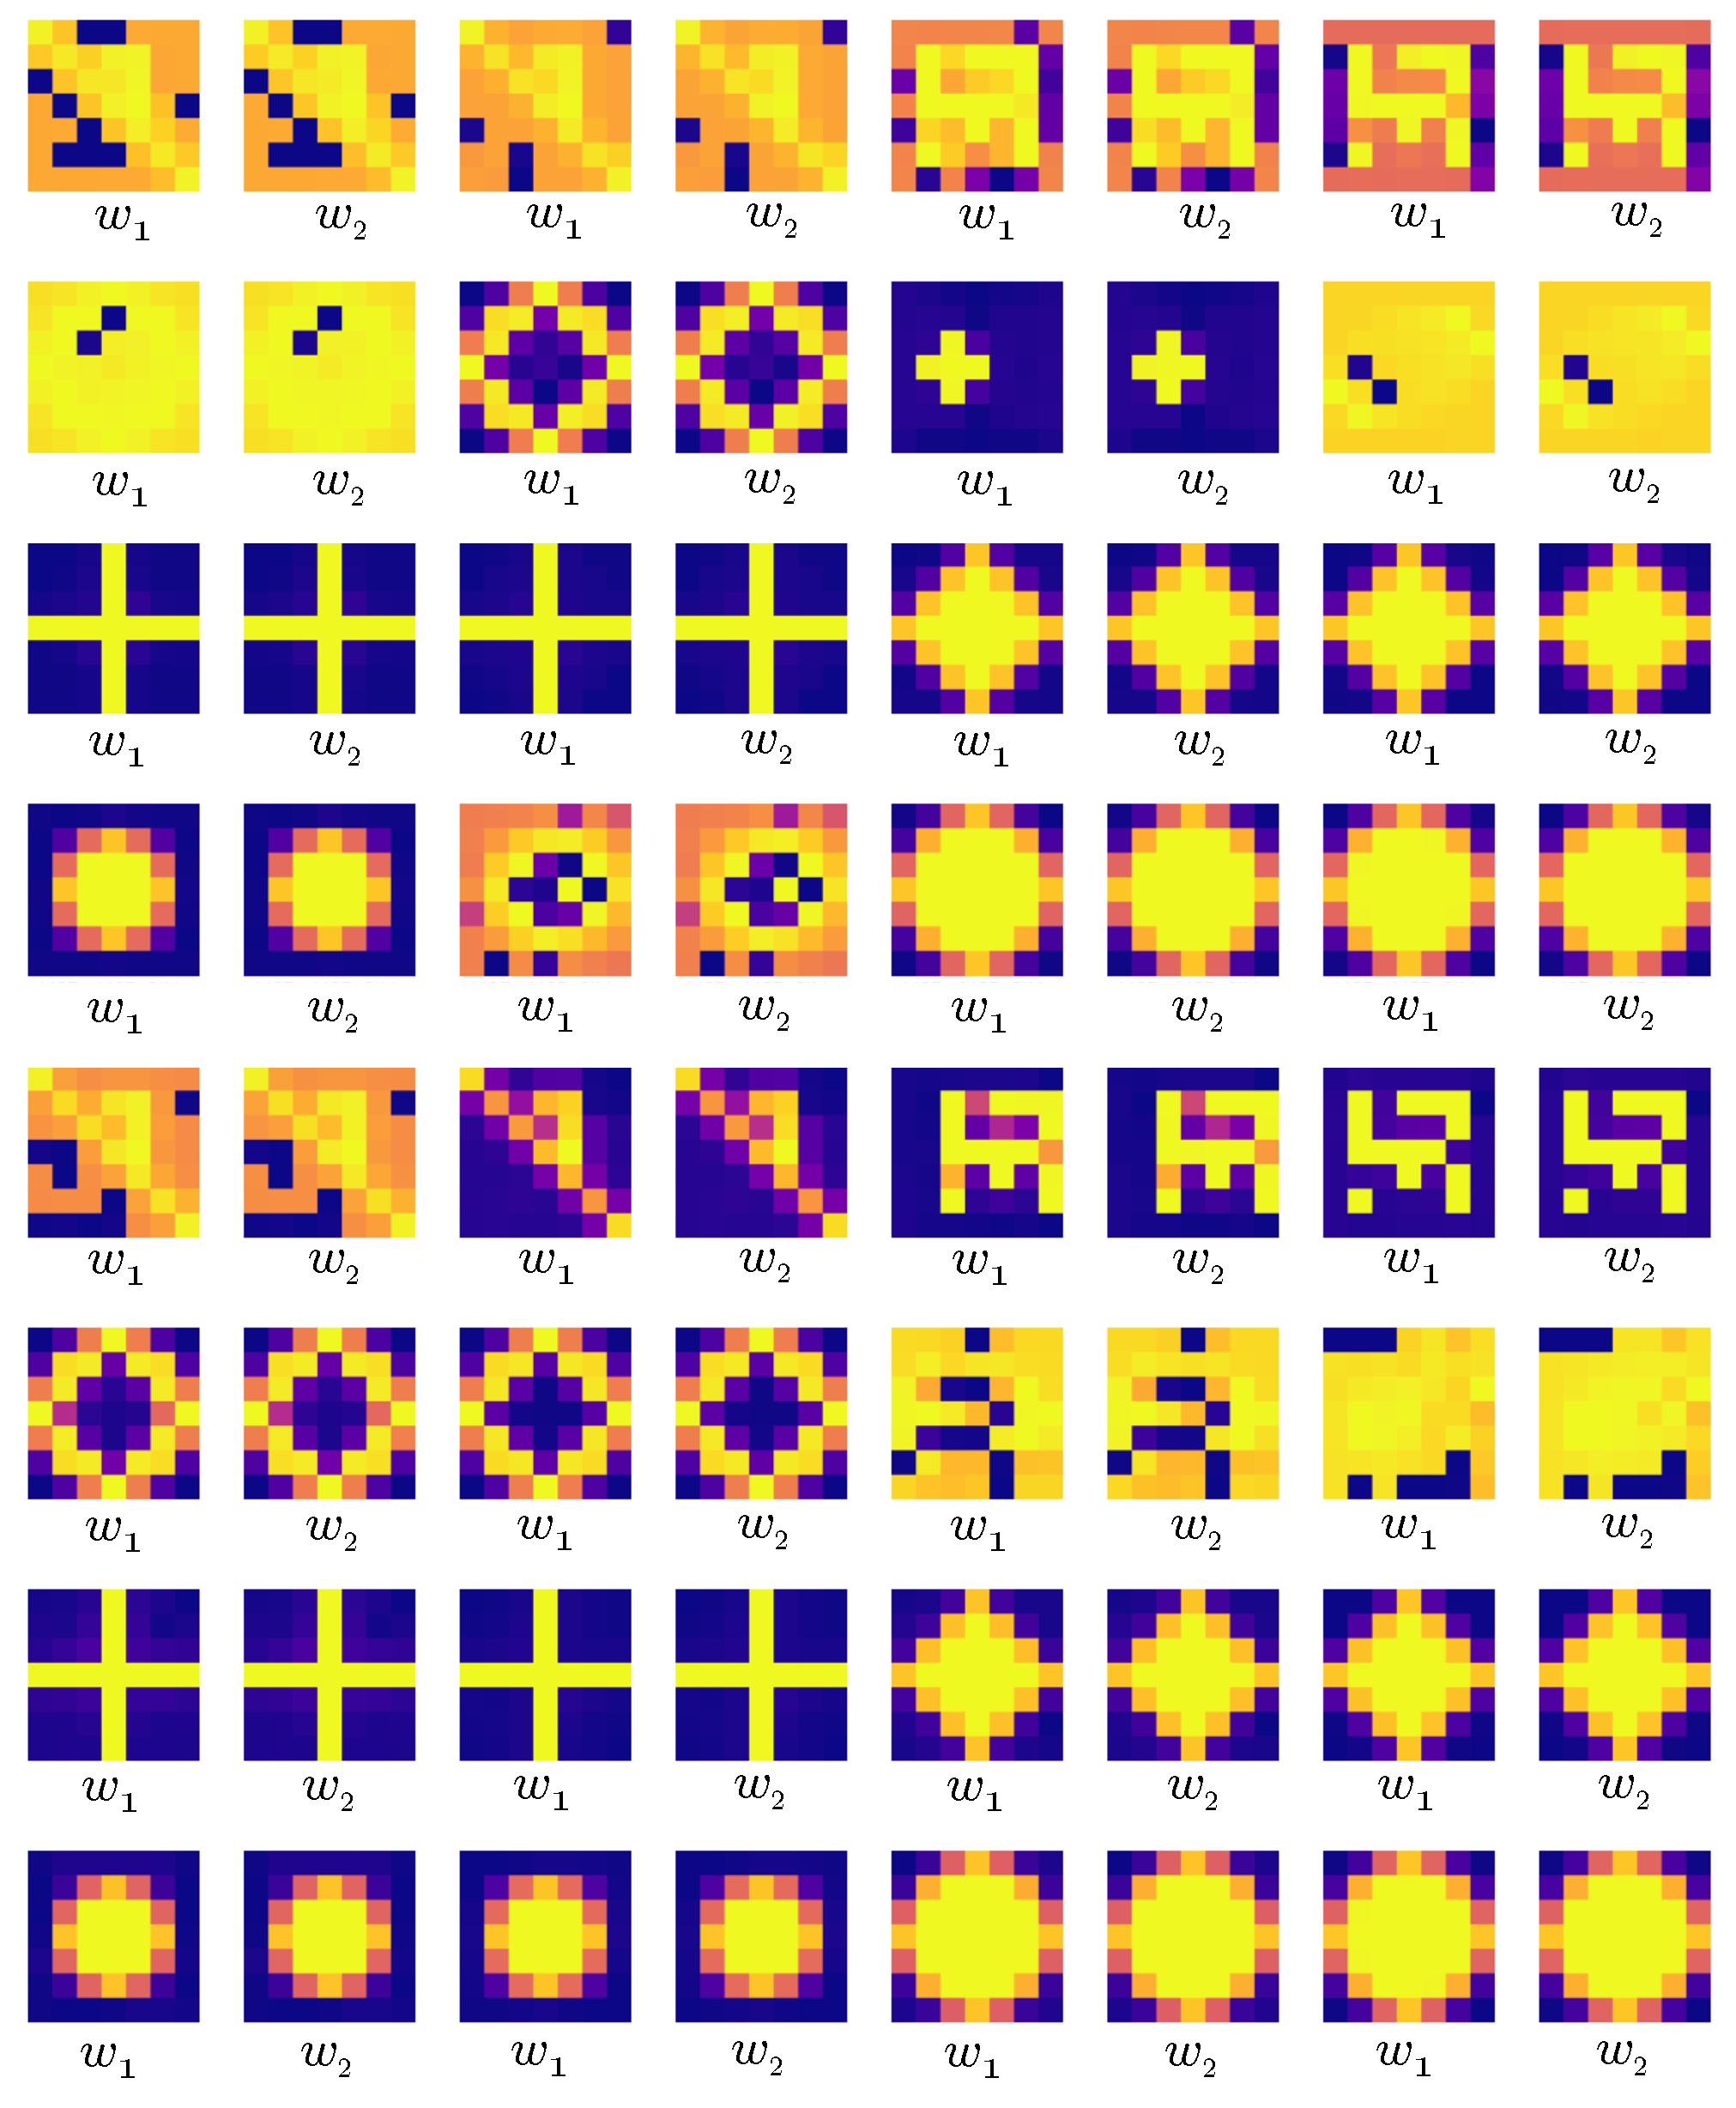
\includegraphics[width=0.31\linewidth]{parts/3-contributions/B-partage_de_poids/figures/quick_visu_STAND.pdf}
          \label{fig:nor2}}\hfill
      \subfigure[Avec la 3ème formulation]{
          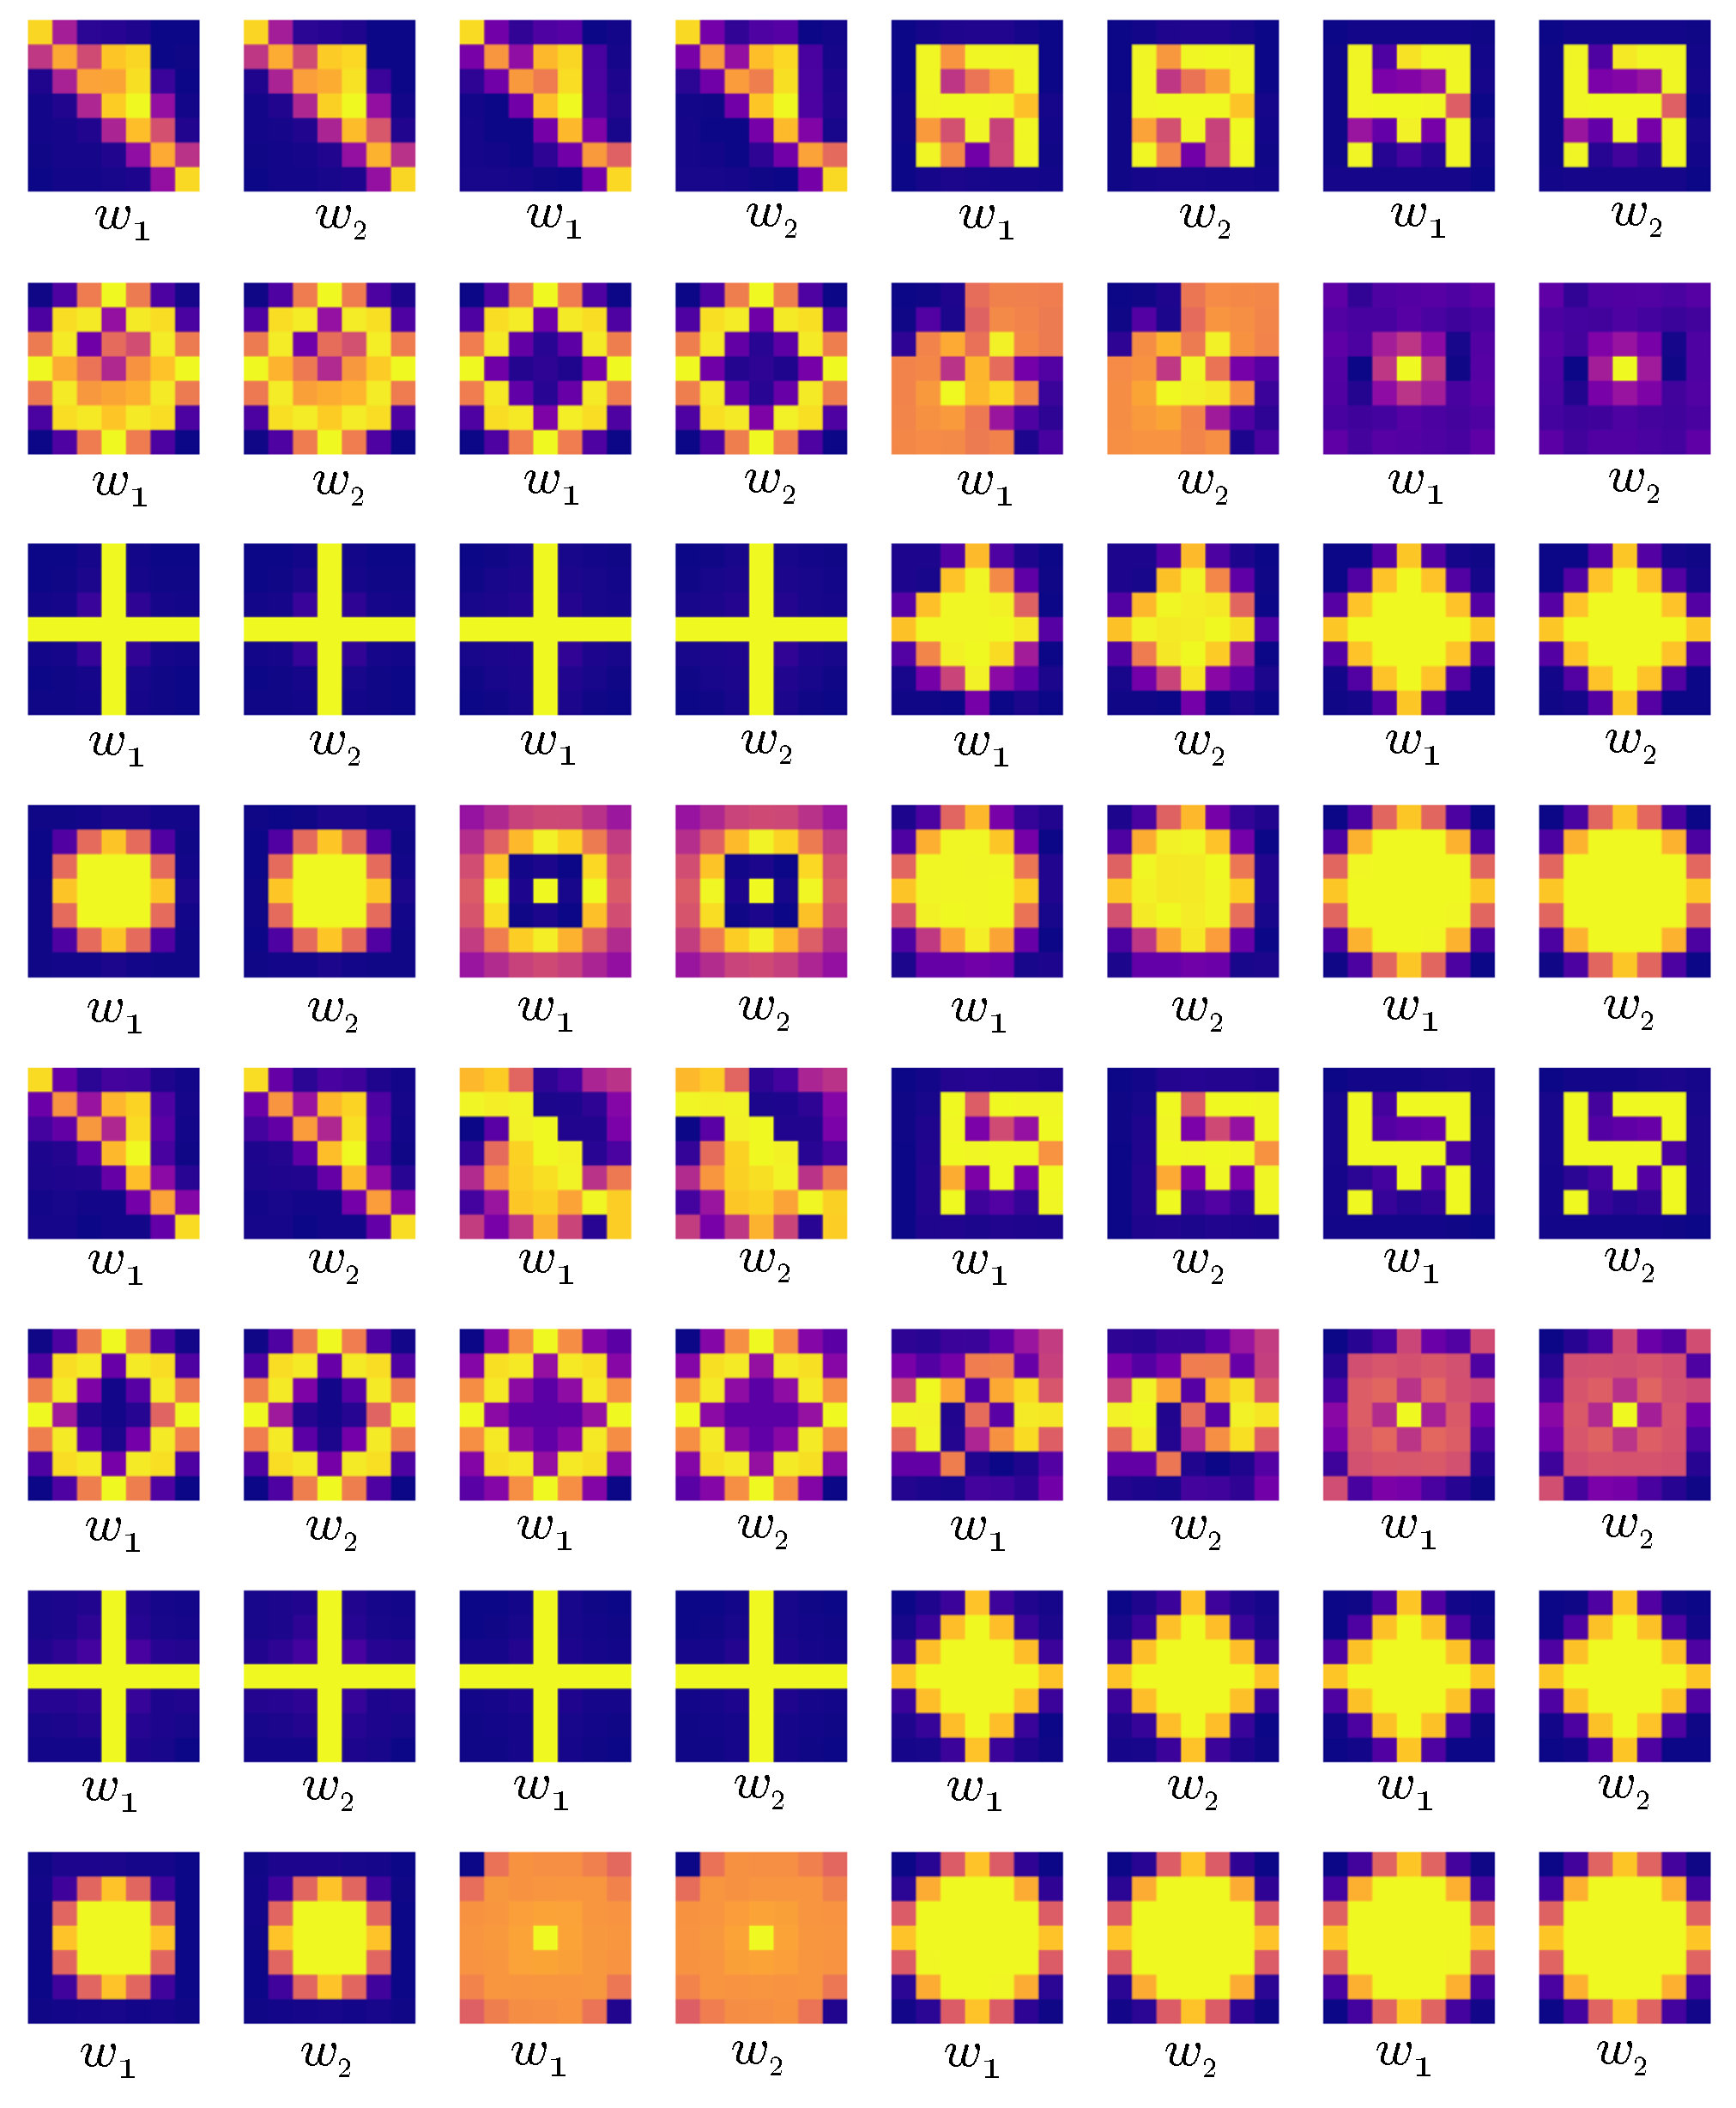
\includegraphics[width=0.31\textwidth]{parts/3-contributions/B-partage_de_poids/figures/quick_visu_TRUE.pdf}
          \label{fig:nor3}}
    \caption{ \centering Forme des noyaux $w_1$ et $w_1$ par paires du réseau $\mathcal{S}$MorphNetTanh à deux couches après convergence, sur un ensemble de 32 expériences, avec dans la \textit{loss} la première formulation de $C_\text{sim}$ (\ref{fig:nor1}), la deuxième (\ref{fig:nor2}) et la troisième (\ref{fig:nor3}).}
    \label{fig:quick_visualisation_contraintes_partage_de_poids}
  \end{center}
\end{figure}

\vspace{-3.5mm}
Sur la figure, chaque emplacement d'un résultat d'une des trois cartes à l'autre représente la même expérience.
On remarque tout de suite le problème avec la première formulation \ref{fig:nor1} basée sur la normalisation (\ref{normalized}) : elle a tendance a binariser les filtres sur certaines expériences (première ligne, les deux premières paires par exemple), en éloignant un unique pixel très bas dans les valeurs (en bleu foncé, jusqu'à -80). Mais cela n'est que visuel, il n'y a pas d'impact sur l'opération car, en dessous d'un certain seuil, toute valeur a le même effet que $-\infty$.
De même pour la seconde formulation \ref{fig:nor2} basée, elle, sur la standardisation (\ref{standardized}). Cependant, elle a tendance à éloigner plusieurs pixels très bas dans les valeurs, plutôt qu'un unique pixel. Quant à la troisième, il n'y a pas ce problème de binarisation, car pas de mise en échelle des gammes. Elle donne les résultats qu'on attendait, similaires à ceux avec la \textit{loss} sans contrainte, mais avec les deux noyaux de chaque paire qui tendent bien vers la même forme. 


%%% Suite page suivante!!

\newpage

On remarque néanmoins que, sur certaines expériences, là où la troisième formulation donne les mêmes mauvais résultats (échecs) de convergence que les expériences sans contrainte dans la \textit{loss} (uniquement la MSE entre les images cibles et les prédictions), les deux autres formulations permettent au réseau de trouver la vraie fonction structurante cible pour ces quelques expériences cibles-là (par exemple, avec le \textit{disk2} en fermeture pour MNIST, dernière ligne et deuxième paire à partir de la gauche).\\

\vspace{-2.0mm}
\noindent Ces bons résultats des deux premières formulations (\ref{Csim1} et \ref{Csim2}), qui surpassent la troisième (\ref{Csim3}) sur ces quelques échecs de convergence, semblent liés au rééchelonnage de la gamme de valeurs des poids $w_1$ et $w_2$, qui fait qu'un éloignement d'une partie des valeurs entraîne une binarisation de ces dernières, qui réduit alors drastiquement la valeur de la contrainte $C_\text{sim}(w_1,w_2)$. Ils pourront être considérés plus tard dans le cadre de l'amélioration de la convergence des réseaux sur ces expériences-là. \\

\vspace{-2.0mm}
\noindent On préfèrera la troisième formulation dans cette optique de partage de poids doux, car seule cette dernière a le comportement que l'on visait initialement, c'est-à-dire faire uniquement tendre les deux noyaux vers la mêmes forme sans créer d'éloignement de valeurs et de binarisation, pour ensuite voir les résultats d'une telle contrainte et estimer si elle permet à elle seule une amélioration de la convergence des réseaux.
